\section{Parallélisation en mémoire partagée (OpenMP)}

\subsection{Stratégie retenue}

\subsubsection{Objectif}

Après la vectorisation (layout SoA), l'objectif du point OpenMP est de réduire le temps noyau
\(K0\) en parallélisant les boucles les plus coûteuses, tout en conservant une sortie benchmark
reproductible (\texttt{METRIC ...}) pour l'analyse de speedup.

\subsubsection{Choix d'architecture}

L'implémentation OpenMP est portée par le backend \texttt{omp+soa}
(\texttt{src/sim/omp\_soa\_backend.cpp}) et sélectionnée via:
\begin{itemize}[leftmargin=*]
  \item \texttt{--exec omp}
  \item \texttt{--layout soa}
\end{itemize}

\subsubsection{Boucles parallélisées}

\begin{enumerate}[leftmargin=*]
  \item \textbf{Évaporation des phéromones (\(K4\)).}
  \texttt{do\_evaporation()} (\texttt{src/pheronome.hpp}) utilise
  \texttt{\#pragma omp parallel for collapse(2) schedule(static)} sur le balayage de grille.
  Les cellules sont indépendantes pendant cette phase.

  \item \textbf{Avance des fourmis (\(K1\)).}
  Dans \texttt{OmpSoaBackend::step}, la boucle sur les indices de fourmis est parallélisée avec
  \texttt{\#pragma omp for schedule(static)}. Pendant la région parallèle, chaque thread:
  \begin{itemize}[leftmargin=*]
    \item met à jour ses fourmis locales (\texttt{x[i], y[i], state[i], seed[i]}),
    \item enregistre les cellules touchées (\texttt{touched\_v1/touched\_v2}),
    \item accumule son \texttt{food\_delta} local.
  \end{itemize}
  Aucune écriture globale directe dans la carte de phéromones n'est faite dans la boucle parallèle.
\end{enumerate}

\subsubsection{Correctness et absence de data races}

Les points sensibles en mémoire partagée sont:
\begin{itemize}[leftmargin=*]
  \item la carte de phéromones (écritures concurrentes potentielles),
  \item le compteur global \texttt{food\_quantity} (incréments concurrents).
\end{itemize}

Le schéma retenu évite ces conflits:
\begin{itemize}[leftmargin=*]
  \item structures locales par thread (\texttt{touched\_v1/touched\_v2}, \texttt{food\_delta}),
  \item fusion après la région parallèle,
  \item replay séquentiel des marquages.
\end{itemize}

\subsubsection{Réduction sparse et robustesse d'ordre}

Après la région parallèle:
\begin{enumerate}[leftmargin=*]
  \item concaténation des vecteurs \texttt{touched} de tous les threads,
  \item tri + \texttt{unique} pour ne garder qu'une fois chaque cellule,
  \item application séquentielle des marques sur la carte globale.
\end{enumerate}

Ce schéma reste cohérent avec un marquage idempotent (politique de fusion par max),
robuste à l'ordre de traitement des fourmis.

\subsubsection{Profilage OpenMP-safe}

Le profilage combine deux niveaux:
\begin{itemize}[leftmargin=*]
  \item \textbf{wall-time} aux frontières des kernels (\(K1\), \(K4\), \(K5\)),
  \item \textbf{work-time} pour \(K2/K3\) (somme du travail interne des threads).
\end{itemize}

En OpenMP, \(K2/K3\) sont accumulés localement par thread puis fusionnés après la région parallèle
(pas d'atomiques dans la boucle chaude). Ainsi:
\begin{itemize}[leftmargin=*]
  \item \(K1\) est un temps mur (comparaison directe de performance),
  \item \(K2/K3\) décrivent la quantité de travail, mais ne doivent pas être lus comme temps mur.
\end{itemize}

\subsection{Protocole expérimental}

Campagnes utilisées:
\begin{itemize}[leftmargin=*]
  \item OpenMP SoA: \texttt{results/test\_openmp\_report\_local/omp/soa/latest}
  \item Référence serial SoA (1 thread): \texttt{results/test\_openmp\_report\_local/serial/soa/latest}
\end{itemize}

Configuration commune:
\begin{itemize}[leftmargin=*]
  \item 1200 itérations, 200 warm-up, donc 1000 itérations mesurées,
  \item mode \texttt{--benchmark --no-render},
  \item 7 répétitions par configuration,
  \item machine: AMD Ryzen 7 5800H (8 coeurs physiques / 16 threads logiques), WSL2,
  \item sweep \(\{1,2,4,8\}\) aligné sur les coeurs physiques.
\end{itemize}

Commande type:
\begin{verbatim}
./scripts/measure_openmp.sh --folder test_openmp_report_local --layout soa --exec omp \
  --threads 1,2,4,8 --iterations 1200 --warmup 200 --reps 7
\end{verbatim}

\subsection{Résultats}

\begin{table}[H]
\centering
\caption{OpenMP SoA: temps noyau et speedup selon le nombre de threads}
\label{tab:omp-speedup}
\begin{tabular}{@{}rrrrr@{}}
\toprule
\textbf{Threads} & \textbf{K0 moyen (ms/iter)} & \textbf{écart-type} & \textbf{Speedup \(S(p)\)} & \textbf{Efficacité \(E(p)=S/p\)} \\
\midrule
1 & 8.684056 & 0.264434 & 1.000000 & 1.0000 \\
2 & 5.539441 & 0.275826 & 1.567677 & 0.7838 \\
4 & 4.612187 & 0.373999 & 1.882850 & 0.4707 \\
8 & 3.564663 & 0.806521 & 2.436151 & 0.3045 \\
\bottomrule
\end{tabular}
\end{table}

\subsubsection{Calcul explicite du speedup mesuré}

Le speedup expérimental est défini par:
\[
S(p)=\frac{T(1)}{T(p)}
\]
où \(T(p)\) est le temps moyen de \(K0\) avec \(p\) threads.
Dans cette section, la référence \(T(1)\) est \textbf{le backend \texttt{omp+soa} à 1 thread}
(pas \texttt{serial+soa}), afin de mesurer strictement l'effet du threading à algorithme constant.

\[
T(1)=8.684056,\quad
T(2)=5.539441,\quad
T(4)=4.612187,\quad
T(8)=3.564663
\]
\[
S(1)=\frac{8.684056}{8.684056}=1.000000
\]
\[
S(2)=\frac{8.684056}{5.539441}=1.567677321 \approx 1.567677
\]
\[
S(4)=\frac{8.684056}{4.612187}=1.882850308 \approx 1.882850
\]
\[
S(8)=\frac{8.684056}{3.564663}=2.436151334 \approx 2.436151
\]

\begin{figure}[H]
  \centering
  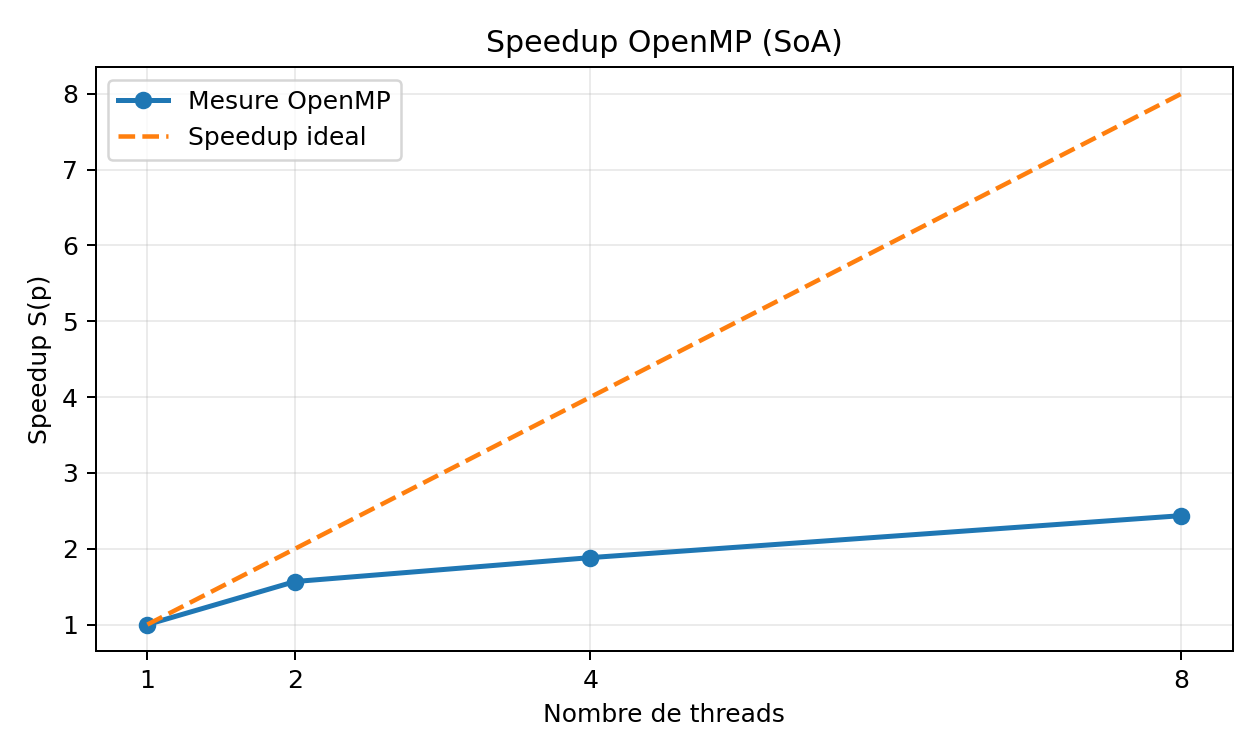
\includegraphics[width=0.82\textwidth]{imgs/openmp/openmp_speedup.png}
  \caption{Speedup mesuré OpenMP (SoA) vs speedup idéal linéaire}
  \label{fig:omp-speedup}
\end{figure}

\begin{figure}[H]
  \centering
  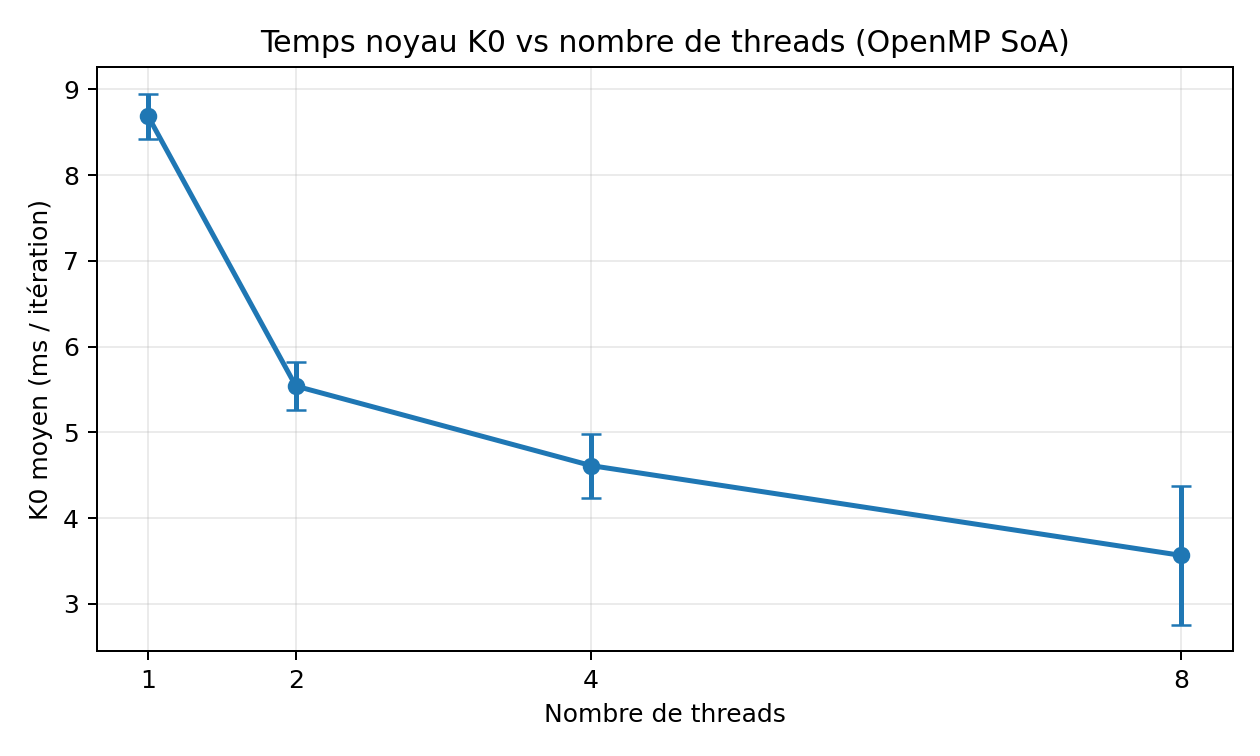
\includegraphics[width=0.82\textwidth]{imgs/openmp/openmp_k0_ms_iter.png}
  \caption{Temps noyau \(K0\) en fonction du nombre de threads (barres d'erreur: écart-type)}
  \label{fig:omp-k0}
\end{figure}

\begin{table}[H]
\centering
\caption{Décomposition du noyau OpenMP SoA (wall-time)}
\label{tab:omp-breakdown}
\begin{tabular}{@{}rrrr@{}}
\toprule
\textbf{Threads} & \textbf{K1 (ms/iter)} & \textbf{K4 (ms/iter)} & \textbf{K5 (ms/iter)} \\
\midrule
1 & 8.014997 & 0.649239 & 0.015685 \\
2 & 5.023505 & 0.400604 & 0.011876 \\
4 & 4.126514 & 0.366018 & 0.014365 \\
8 & 3.219344 & 0.317306 & 0.014992 \\
\bottomrule
\end{tabular}
\end{table}

\begin{figure}[H]
  \centering
  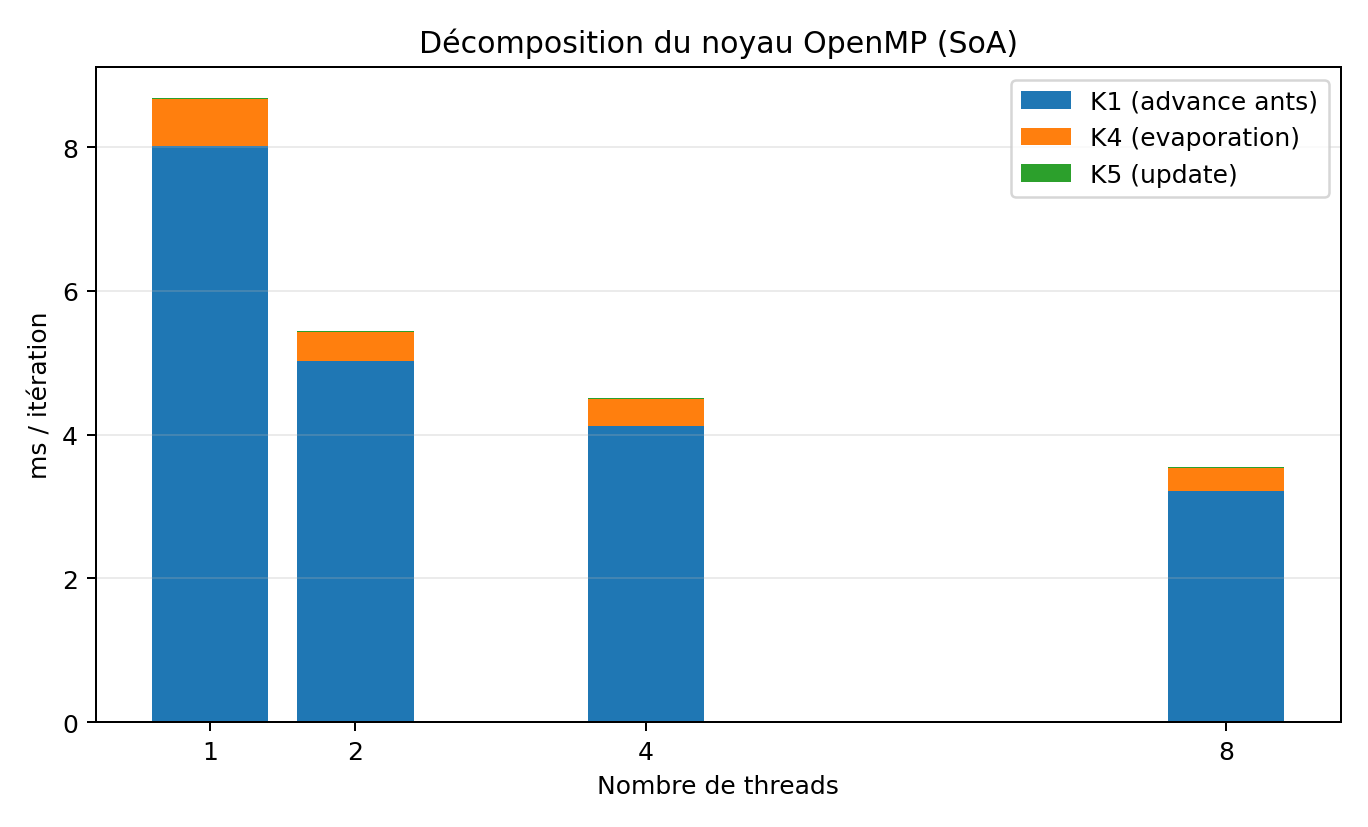
\includegraphics[width=0.84\textwidth]{imgs/openmp/openmp_kernel_breakdown.png}
  \caption{Décomposition \(K1/K4/K5\) du noyau OpenMP SoA}
  \label{fig:omp-breakdown}
\end{figure}

\begin{table}[H]
\centering
\caption{Work-time interne OpenMP SoA (\(K2\), \(K3\))}
\label{tab:omp-k23-worktime}
\begin{tabular}{@{}rrr@{}}
\toprule
\textbf{Threads} & \textbf{K2 work-time (ms/iter)} & \textbf{K3 work-time (ms/iter)} \\
\midrule
1 & 3.640941 & 0.532093 \\
2 & 3.275849 & 0.587566 \\
4 & 3.503250 & 0.777031 \\
8 & 3.399851 & 0.815067 \\
\bottomrule
\end{tabular}
\end{table}

\subsubsection{Vérifications empiriques de correctitude}

En complément de l'argument ``absence de races'', on vérifie deux invariants simples:
\begin{itemize}[leftmargin=*]
  \item \texttt{food\_quantity} monotone non décroissante (\texttt{food\_monotonic\_ok=1}),
  \item stabilité d'indicateurs globaux de phéromones entre 1 et 8 threads (même seed).
\end{itemize}

\begin{table}[H]
\centering
\caption{Checks de correctitude OpenMP (5000 itérations, warmup 500, seed 2026)}
\label{tab:omp-correctness-checks}
\begin{tabular}{@{}lrr@{}}
\toprule
\textbf{Métrique} & \textbf{OMP 1 thread} & \textbf{OMP 8 threads} \\
\midrule
\texttt{food\_monotonic\_ok} & 1 & 1 \\
\texttt{food\_quantity\_final} & 1556 & 1556 \\
\texttt{phen\_v1\_sum} & 2989.08 & 2989.08 \\
\texttt{phen\_v2\_sum} & 16321.2 & 16321.2 \\
\texttt{phen\_v1\_max} & 1.0 & 1.0 \\
\texttt{phen\_v2\_max} & 1.0 & 1.0 \\
\bottomrule
\end{tabular}
\end{table}

\subsection{Analyse et discussion des résultats}

Le speedup croît bien avec le nombre de threads, mais reste loin de la droite idéale:
\[
S(8)=2.4362 \quad (\text{vs idéal } 8.0)
\]

\begin{itemize}[leftmargin=*]
  \item \textbf{Lecture Amdahl.} Avec \(S(8)=2.436151\), on obtient:
  \[
  f \approx \frac{8/S(8)-1}{7}\approx 0.33,\qquad S_{\max}\approx \frac{1}{f}\approx 3.06.
  \]
  Le plafonnement observé autour de \(2.4\) est cohérent avec cette borne.
\end{itemize}

\begin{itemize}[leftmargin=*]
  \item \textbf{K4 (évaporation), comportement memory-bound.}
  \[
  K4:\ 0.649239 \rightarrow 0.317306\ \text{ms/iter (1 $\to$ 8)} \approx -51.1\%.
  \]
  Le gain est net mais non linéaire, typique d'une limite de bande passante mémoire.
\end{itemize}

\begin{itemize}[leftmargin=*]
  \item \textbf{K1 (avance des fourmis), gain significatif mais borné.}
  \[
  K1:\ 8.014997 \rightarrow 3.219344\ \text{ms/iter (1 $\to$ 8)} \approx -59.8\%.
  \]
  La phase de fusion sparse (\texttt{concat}, \texttt{sort+unique}, replay) reste partiellement
  séquentielle et freine la scalabilité.
\end{itemize}

\begin{itemize}[leftmargin=*]
  \item \textbf{Interprétation de \(K2/K3\).}
  Les valeurs \(K2/K3\) sont des work-times: elles décrivent le volume de travail interne et
  l'évolution de la granularité, mais ne s'additionnent pas directement en temps mur.
\end{itemize}

\begin{itemize}[leftmargin=*]
  \item \textbf{Comparaison \texttt{serial+soa} vs \texttt{omp+soa} à 1 thread.}
  La référence serial locale vaut \(K0=7.924494\) ms/iter, contre \(8.684056\) ms/iter pour
  \texttt{omp+soa} à 1 thread (\(+9.6\%\)). Cet écart vient du coût structurel propre au backend
  OMP (buffers touched, merge, dedup, replay), indépendamment du speedup de threading.
\end{itemize}

\noindent\textbf{Bilan.}
\begin{itemize}[leftmargin=*]
  \item accélération mesurable et reproductible (\(S(8)\approx 2.44\)),
  \item \(K4\) limité principalement par la mémoire,
  \item \(K1\) limité par la fusion sparse post-parallèle.
\end{itemize}
